\documentclass[12pt, a4paper, twoside]{article}

%% Preamble
\usepackage{pdfpages}           % Para incluir PDFs
\usepackage{graphicx}           % Para gráficos
\usepackage{subfiles}           % Para manejar subarchivos
\usepackage{hyperref}           % Para enlaces
\usepackage{listings}           % Para código fuente (ajusta lenguaje)
\usepackage{verbatim}
\usepackage[backend=bibtex,style=numeric]{biblatex} % Para citas numéricas
\addbibresource{references.bib} % Cargar archivo .bib
\usepackage{url}
\usepackage{float}


\usepackage{geometry}           % Para ajustar márgenes

% Ajustes de márgenes
\geometry{
	left=3cm,       % Margen izquierdo
	right=3cm,      % Margen derecho
	top=2.5cm,      % Margen superior
	bottom=2.5cm,   % Margen inferior
	headheight=15pt, % Altura del encabezado
	twoside          % Para documentos a dos caras
}


\graphicspath{{images/}{../images/}} % Ruta para imágenes

\begin{document}
	
	%% Cover
	
\includepdf[noautoscale=true, width=\paperwidth]{cover.pdf}
	
	%% Title
	\clearpage
	\setcounter{page}{1}
	
\includepdf[noautoscale=true, width=\paperwidth]{title.pdf}
	
	%%%%%%%%%%%%%%%%%%%%%%%%%%%%%%%%%%%%%%%%%%%%%%%%%%%%%%%%%%%%%%%%%%%%%%%%%%%
	
	% Índice automático
	\tableofcontents
	\newpage
	
	\section{Introducción}
	
	Este documento es una continuación de las fases anteriores del proyecto, donde se desarrollaron el \textbf{diseño conceptual y lógico} de un almacén de datos basado en la información proporcionada por la \textit{Base de Datos de Investigación Colaborativa eICU} \cite{eICU2024}, y la \textbf{integración de datos} mediante un proceso de Extracción, Transformación y Carga (ETL). Para la creación de un almacén enfocado a \textbf{pacientes con patologías respiratorias}.
	
	En esta fase, se busca construir un \textbf{cubo multidimensional} utilizando los datos del almacén previamente desarrollado,	En el ámbito hospitalario, la creación de un cubo multidimensional ofrece ventajas al permitir analizar datos clínicos complejos de manera ágil. Posteriormente se realizarán consultas en \textit{MDX} (Multidimensional Expressions) sobre dicho cubo.  Permitiendo extraer información de manera eficiente al navegar por las dimensiones y medidas del cubo.

	
	Además, se describirán los problemas encontrados durante el desarrollo y las soluciones aplicadas, asegurando que las consultas generen resultados útiles para el análisis de datos.
	
	
	
	\section{Objetivos}
	
	Los objetivos principales de este informe son los siguientes:
	
	\begin{itemize}
		\item Realizar las correcciones pertinentes en el proceso ETL que permitan el desarrollo del cubo muldimensional.
		\item Implementar un cubo multidimensional adaptado para el análisis de \textbf{pacientes con patologías respiratorias}.
		\item Desarrollar al menos 8 consultas en \textit{MDX} que exploren diferentes dimensiones y hechos del cubo, aplicando funciones avanzadas cuando sea necesario.
		\item Documentar de manera clara y replicable el proceso de creación del cubo multidimensional y las consultas \textit{MDX}, proporcionando instrucciones detalladas para su ejecución.
		\item Describir los problemas encontrados durante el desarrollo del cubo y las consultas, y detallar las soluciones empleadas.
	\end{itemize}
	
	
	 
	
	\section{\textbf{Modificación del almacén de datos}}
	
	\begin{itemize}
		\item Se \textbf{eliminaron las columnas} `Age` y `PatientUnitStayID` de la tabla de pacientes.
		\item Se \textbf{seleccionaron únicamente los pacientes únicos}, conservando solo su primera aparición en la base de datos. Anteriormente, el número total de pacientes era 1849, pero después de aplicar esta modificación, el total es de 1841, lo que es correcto.
		\item Para el \textbf{tiempo}, se utilizó la cláusula `DISTINCT` para evitar \textbf{fechas duplicadas en el ingreso}.
		\item Para la \textbf{información de diagnóstico}, se extrajo el primer valor de la columna `DiagnosisString` (primera dimensión). La consulta SQL utilizada para obtener los datos de diagnóstico de la base de datos fue la siguiente:
		\begin{verbatim}
			SELECT 
			DiagnosisID,
			PatientUnitStayID,
			ActiveUponDischarge,
			DiagnosisOffset,
			ICD9Code,
			DiagnosisPriority,
			SUBSTRING(DiagnosisString, 1, CHARINDEX('|'
			, DiagnosisString + '|') - 1) AS FirstDiagnosis
			FROM Diagnosis;
		\end{verbatim}
		\item Se \textbf{corrigió la creación de las tablas intermedias} para las relaciones `NxM`. Anteriormente, se utilizaba como \textbf{origen de datos la tabla `Diagnosis`} de la base de datos en lugar de la del `Data Warehouse`. Posteriormente, se realizaba un \textbf{`lookup` con `IngresoUCI`} utilizando el `patientID\_og`.
		\item Se \textbf{realizó una transformación en la columna `Age`}, cambiando su tipo de dato de `string` a `integer` para permitir su uso en consultas. Durante este proceso, se transformó el valor `'> 89'` a `90` por defecto. La consulta SQL utilizada para obtener los datos de la tabla `Patient` en la base de datos fue la siguiente:
		\begin{verbatim}
			SELECT 
			T.TiempoID,
			P.UniquePID,
			H.HospitalID,
			I.HospitalDischargeOffset,
			I.PatientHealthSystemStayID,
			I.PatientUnitStayID,
			CASE 
			WHEN I.Age = '> 89' THEN 90                      
			-- Cambiar "> 89" por 90
			WHEN ISNUMERIC(I.Age) = 1 THEN CAST(I.Age AS INT) 
			-- Convertir valores numéricos a INT
			ELSE NULL                                       
			-- Manejar otros casos como NULL
			END AS AgeInt
			FROM [eICU Collaborative Research Database].dbo.Patient I
			LEFT JOIN prueba.dbo.Paciente P ON I.uniquePID = P.uniquePID_og
			LEFT JOIN prueba.dbo.Hospital H ON I.HospitalID = H.hospitalID_og
			LEFT JOIN prueba.dbo.Tiempo T 
			ON I.HospitalDischargeYear = T.HospitalDischargeYear 
			AND I.HospitalDischargeTime24 = T.HospitalDischargeTime24;
		\end{verbatim}
	\end{itemize}
	
		
	
\section{\textbf{Creación del cubo}}

\subsection{\textbf{Orígenes de datos}}

Para la \textbf{creación del cubo}, iniciaremos el proceso estableciendo la conexión con nuestra base de datos:

\begin{figure}[H]
	\centering
	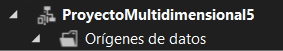
\includegraphics[width=0.5\textwidth]{image/origenDatos}
	\caption{\textbf{Origen de datos}}
	\label{fig:1}
\end{figure}

A continuación, procederemos a \textbf{establecer la conexión con la base de datos}, donde especificaremos el proveedor a utilizar, como se muestra en la Figura \ref{fig:2}. Dado que nuestro servidor se encuentra en el entorno local, se debe indicar únicamente `.` como la dirección del servidor. Es crucial, \textbf{y se debe prestar especial atención}, que la autenticación se configure utilizando \textbf{SQL Server Authentication}. Esto permitirá especificar el nombre de usuario como `sa` y la contraseña asociada, que en este caso será `Almacenes`. Finalmente, seleccionaremos la base de datos correspondiente, que en este escenario es `prueba`, como se ilustra en la Figura \ref{fig:2}.

\begin{figure}[H]
	\centering
	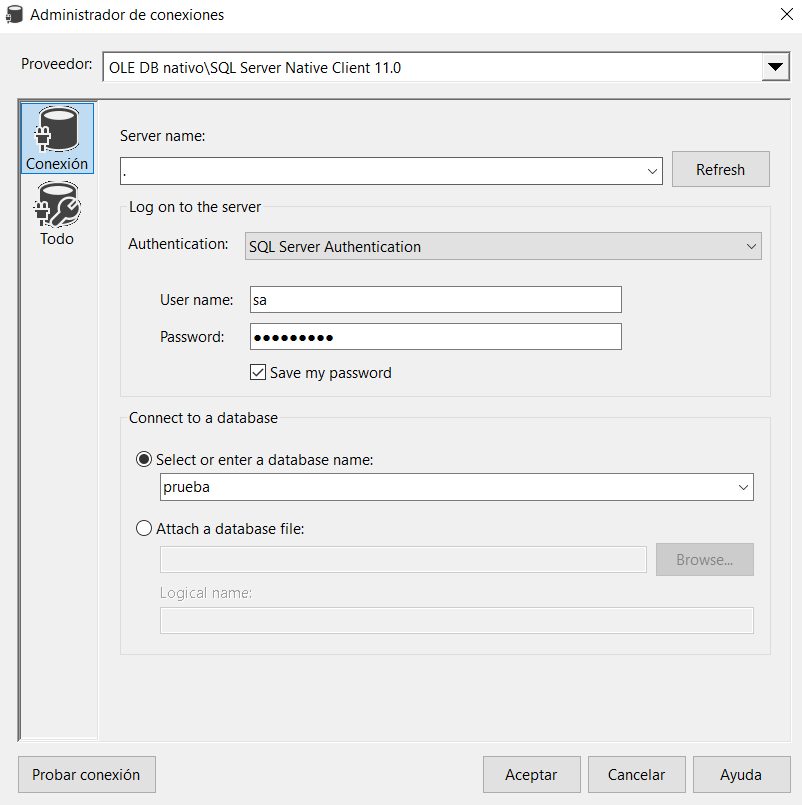
\includegraphics[width=0.7\textwidth]{image/conexion}
	\caption{\textbf{Conexión de datos}}
	\label{fig:2}
\end{figure}

Una vez realizados los pasos anteriores, procederemos a hacer clic derecho sobre las \textbf{vistas del origen de datos} y seleccionaremos la opción "Nueva Vista". Esto nos mostrará todos los orígenes de datos disponibles, siendo en este caso solo la base de datos "Prueba", como se muestra en la Figura \ref{fig:4}.

\begin{figure}[H]
	\centering
	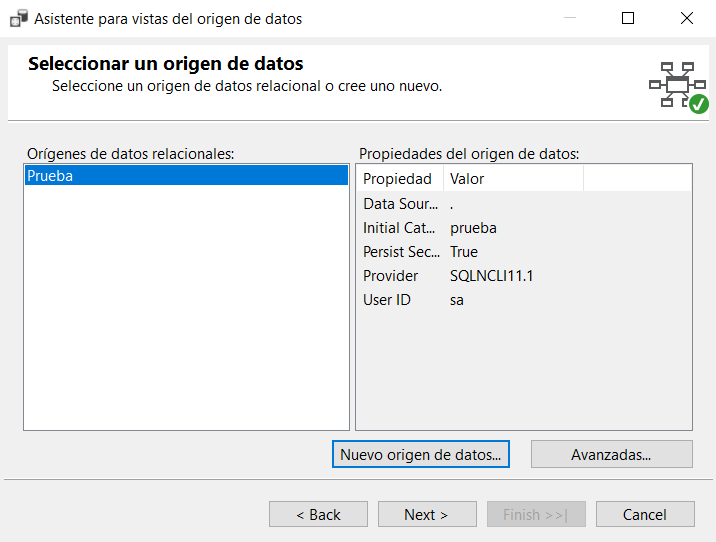
\includegraphics[width=0.7\textwidth]{image/vistaOrigenConexion}
	\caption{\textbf{Vista origen conexión de datos}}
	\label{fig:4}
\end{figure}

A continuación, haremos clic en "Next".

En la siguiente pantalla que aparecerá, como se muestra en la Figura \ref{fig:5}, seleccionaremos el \textbf{botón señalado en rojo}. Esto nos permitirá incluir \textbf{todas las tablas en la vista} para garantizar que el almacén de datos esté completo. Luego, seleccionaremos "Next".

\begin{figure}[H]
	\centering
	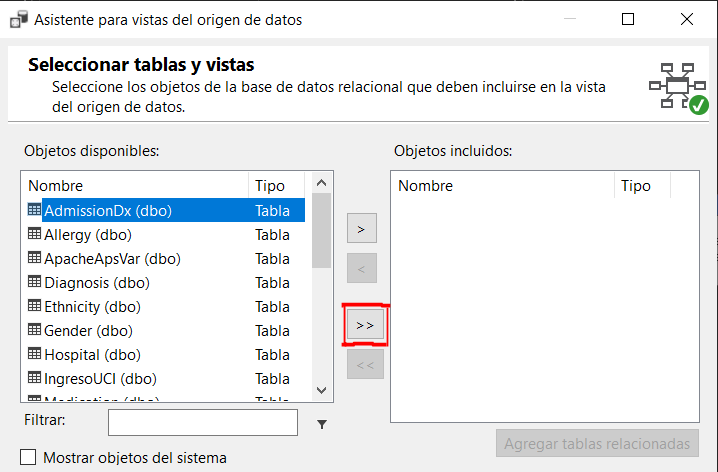
\includegraphics[width=0.7\textwidth]{image/seleccionTablas}
	\caption{\textbf{Selección de tablas}}
	\label{fig:5}
\end{figure}

Posteriormente, aparecerá una nueva pantalla donde podremos \textbf{visualizar lo que contendrá la vista} y, por ende, con qué elementos podremos operar en el cubo, como se muestra en la Figura \ref{fig:6}.

\begin{figure}[H]
	\centering
	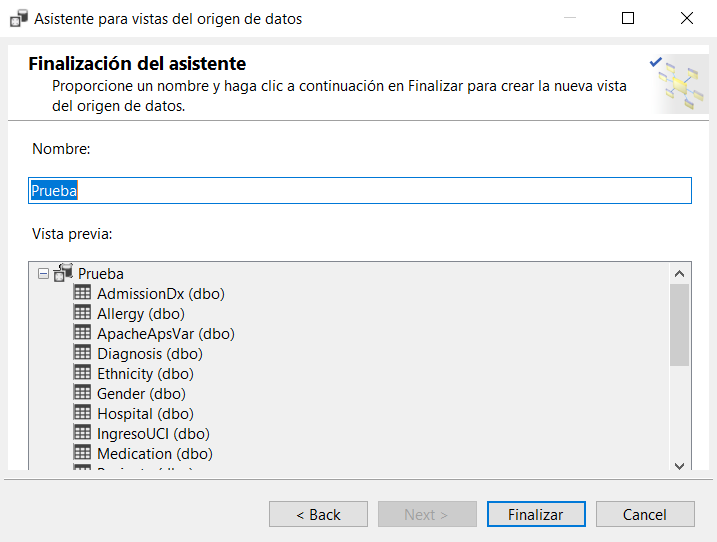
\includegraphics[width=0.7\textwidth]{image/asistenteVista}
	\caption{\textbf{Vista finalización}}
	\label{fig:6}
\end{figure}

Una vez revisado todo, seleccionaremos "Finalizar" como se muestra en la Figura \ref{fig:6}.

Al hacer \textbf{doble clic en la vista recién creada}, podremos ver que contiene todas las tablas que teníamos en nuestro diagrama de SQL Server Management, como se ilustra en la Figura \ref{fig:7}.

\begin{figure}[H]
	\centering
	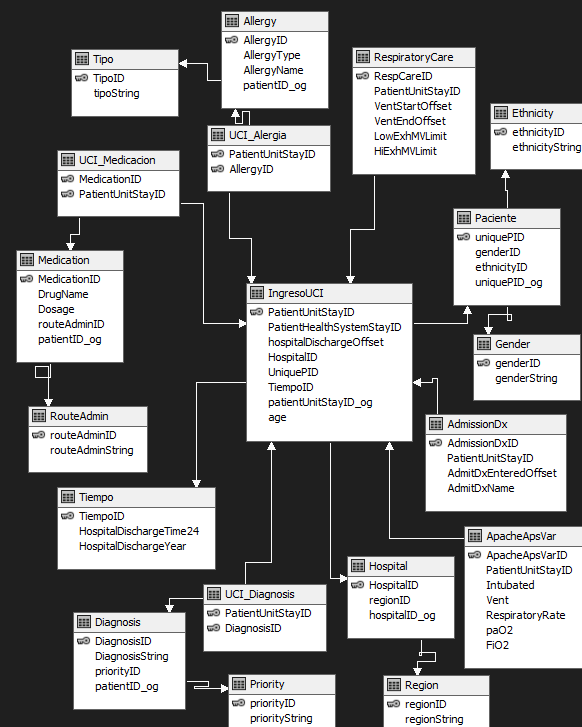
\includegraphics[width=1\textwidth]{image/vista_origenes_datos}
	\caption{\textbf{Vista}}
	\label{fig:7}
\end{figure}

\subsection{\textbf{Crear el cubo}}

Una vez que la \textbf{vista esté configurada}, podemos proceder a \textbf{crear el cubo}. Para ello, haremos clic derecho sobre el proyecto y seleccionaremos "Nuevo Cubo". En la ventana emergente, elegiremos la opción \textbf{"Usar tablas existentes"}, tal como se muestra en la Figura \ref{fig:9}.

\begin{figure}[H]
	\centering
	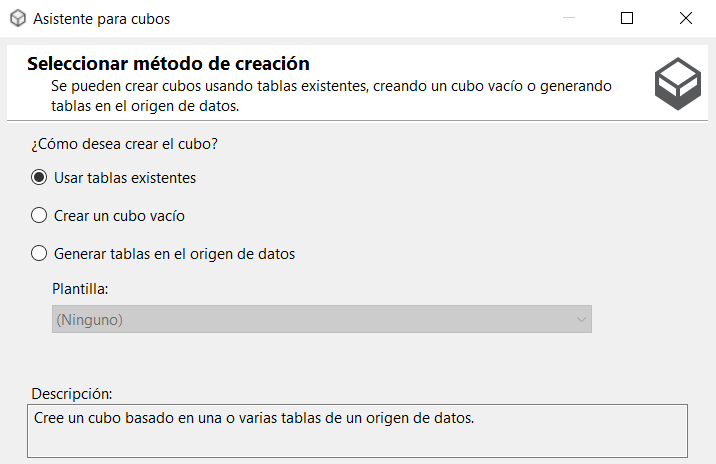
\includegraphics[width=1\textwidth]{image/crearCubo}
	\caption{\textbf{Vista}}
	\label{fig:9}
\end{figure}

Luego, haremos clic en "Next" y aparecerá una pantalla como la que se muestra en la Figura \ref{fig:10}.

\begin{figure}[H]
	\centering
	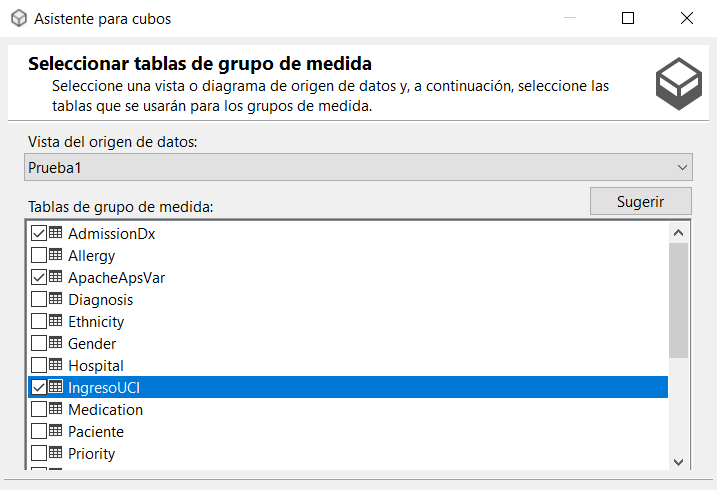
\includegraphics[width=1\textwidth]{image/seleccionTablasCubo}
	\caption{\textbf{Selección tablas del Cubo}}
	\label{fig:10}
\end{figure}

En esta pantalla, seleccionaremos únicamente aquellas \textbf{tablas que tengan una relación de tipo 1 a N} con la tabla de hechos, donde N representa las tablas relacionadas y 1 es la tabla de hechos. Esto incluye las tablas \textit{AdmissionDx}, \textit{ApacheApsVar}, \textit{RespiratoryCare}, así como las tablas intermedias (\textit{UCI\_Medicacion}, \textit{UCI\_Diagnosis} y \textit{UCI\_Alergia}) resultantes de las relaciones NxM entre las tablas \textit{Medication}, \textit{Diagnosis} y \textit{Allergy}.

Si hemos seguido correctamente los pasos anteriores, el resultado será similar al mostrado en la Figura \ref{fig:8}.

\begin{figure}[H]
	\centering
	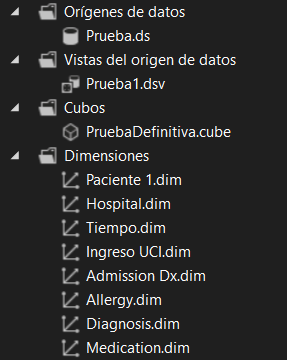
\includegraphics[width=0.5\textwidth]{image/loquellevamos}
	\caption{\textbf{Proyecto Multidimensional}}
	\label{fig:8}
\end{figure}

\textbf{Cabe destacar que las dimensiones se generan automáticamente a partir de la creación del cubo.}

	
\subsection{Modificación de las dimensiones}

Ahora procederemos con la modificación de las dimensiones para su uso correcto en el cubo.

Si damos doble clic en la dimensión \texttt{Paciente} y nos vamos al apartado de "Estructura de dimensión", veremos en la columna de atributos las claves almacenadas en \texttt{Paciente}, como se muestra en la Figura \ref{fig:11}. Ahora, lo que haremos será crear jerarquías para utilizarlas posteriormente en las consultas.

Nota: \textbf{Para cada cambio relacionado con las dimensiones, será necesario procesar y actualizar la dimensión}. Para ello, tendremos que estar en Browser o Explorador en Español.

\subsubsection{Ethnicity - Paciente}

En el caso de \texttt{Paciente}, teníamos una doble jerarquía. Por un lado, era el género y por otro, la etnia. Para crear estas jerarquías, arrastraremos la clave de la jerarquía que queramos empezar, ya sea \texttt{GenderID} o \texttt{EthnicityID}, al área donde aparece "Jerarquías". Luego, arrastraremos la clave \texttt{UniquePID}. Esto dará lugar a dos jerarquías similares a las mostradas en la Figura \ref{fig:11}.

\begin{figure}[H]
	\centering
	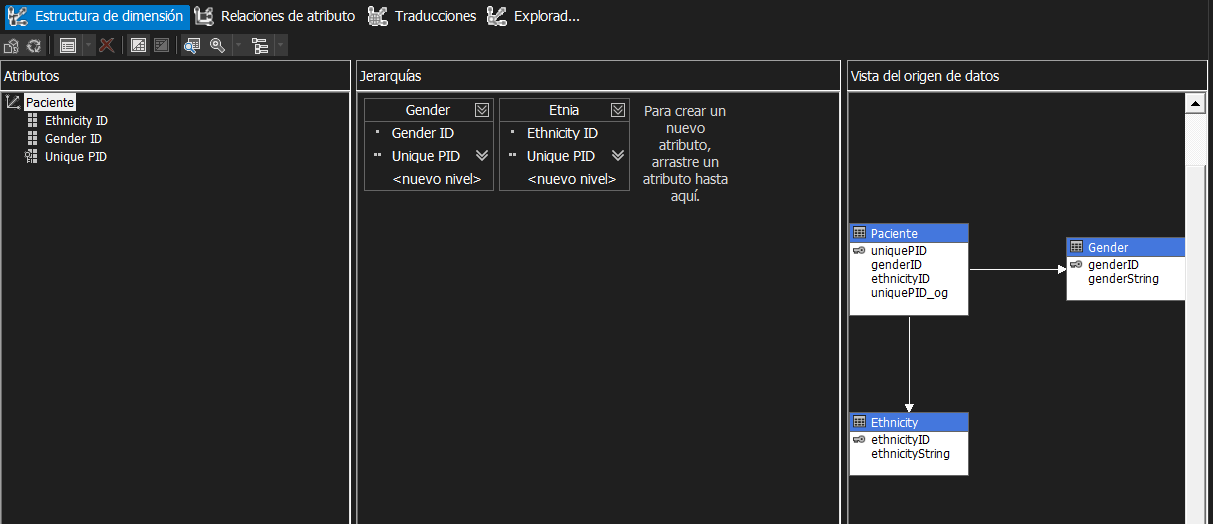
\includegraphics[width=1\textwidth]{image/dimPaciente}
	\caption{Dimensión Paciente}
	\label{fig:11}
\end{figure}

Posteriormente, para que las jerarquías se entiendan correctamente y no se utilicen solo ID's, será necesario hacer los siguientes cambios.

Daremos clic en \texttt{EthnicityID} y en el recuadro inferior derecho nos aparecerán las propiedades de dicho atributo, como se muestra en la Figura \ref{fig:12}.

\begin{figure}[H]
	\centering
	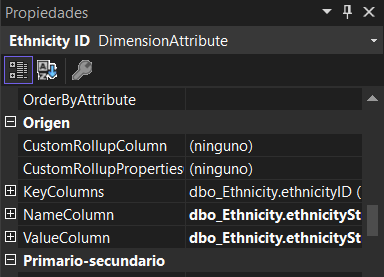
\includegraphics[width=1\textwidth]{image/EthnicityID}
	\caption{EthnicityID}
	\label{fig:12}
\end{figure}

Nos iremos al apartado \textbf{NameColumn}, le daremos a los tres puntos y nos saldrá una ventana parecida a la Figura \ref{fig:13}: 

\begin{figure}[H]
	\centering
	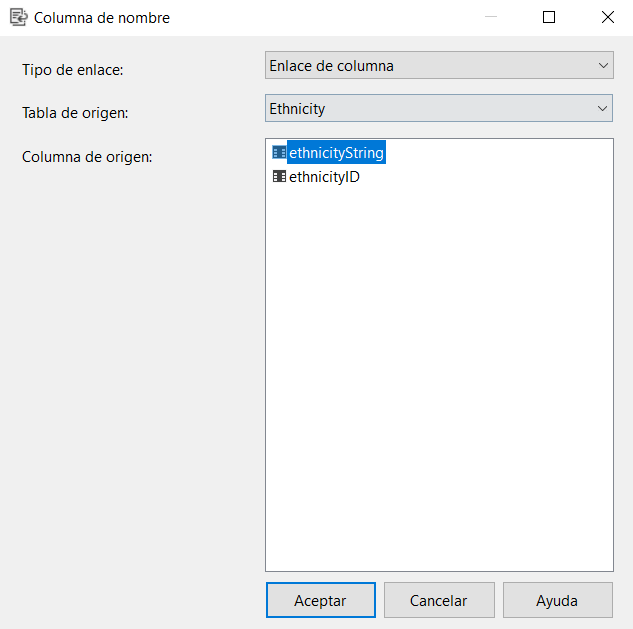
\includegraphics[width=1\textwidth]{image/EthnicityID2}
	\caption{EthnicityID}
	\label{fig:13}
\end{figure}

Ahora seleccionaremos \texttt{ethnicityString} como \textbf{NameColumn}. Ya por último, siguiendo en el apartado de propiedades, tendremos que poner en \textbf{ValueColumn} el valor \texttt{ethnicityString}, también, ya que no queremos realmente que las jerarquías sean por el ID sino por el string asociado a ellos.

Haremos exactamente el mismo proceso para el resto de tablas, \textbf{exceptuando Tiempo}, que la comentaré más tarde.

\subsubsection{Gender - Paciente}

\textbf{ValueColumn} y \textbf{NameColumn}:

\begin{figure}[H]
	\centering
	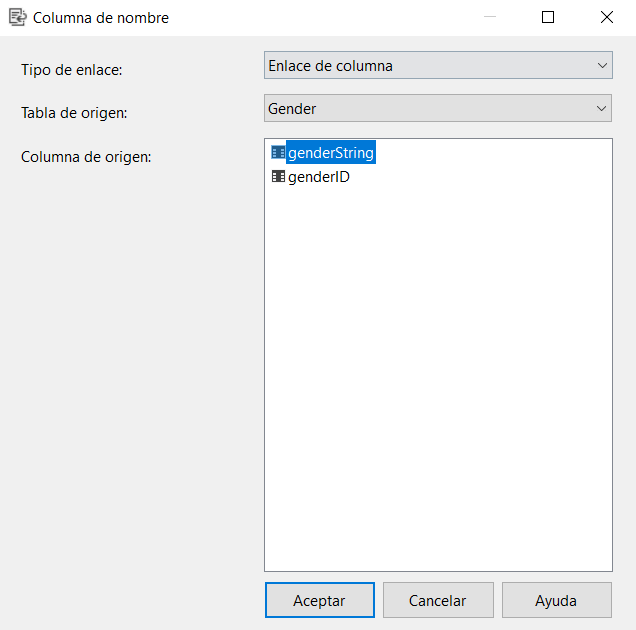
\includegraphics[width=1\textwidth]{image/GenderID}
	\caption{GenderID}
	\label{fig:14}
\end{figure}

Seleccionamos \texttt{genderString}.

\subsubsection{Hospital}

\textbf{Jerarquía:}

\begin{figure}[H]
	\centering
	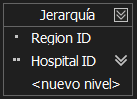
\includegraphics[width=0.5\textwidth]{image/JRegion}
	\caption{Jerarquía de Region}
	\label{fig:15}
\end{figure}

\textbf{ValueColumn} y \textbf{NameColumn}:

\begin{figure}[H]
	\centering
	\includegraphics[width=1\textwidth]{image/RegionID}
	\caption{RegionID}
	\label{fig:16}
\end{figure}

Seleccionamos \texttt{regionString}. Como no teníamos ningún nombre de hospital, lo que tendremos serán las regiones y todos los IDs de los hospitales asociados a esa región.

\subsubsection{IngresoUCI}

\textbf{Jerarquía:}

\begin{figure}[H]
	\centering
	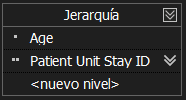
\includegraphics[width=0.5\textwidth]{image/JIngresoUCI}
	\caption{Jerarquía de IngresoUCI}
	\label{fig:17}
\end{figure}

\subsubsection{Allergy}

\textbf{Jerarquía:}

\begin{figure}[H]
	\centering
	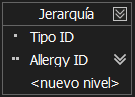
\includegraphics[width=0.5\textwidth]{image/JAlergia}
	\caption{Jerarquía de Alergia}
	\label{fig:18}
\end{figure}

\textbf{ValueColumn} y \textbf{NameColumn}:

\begin{figure}[H]
	\centering
	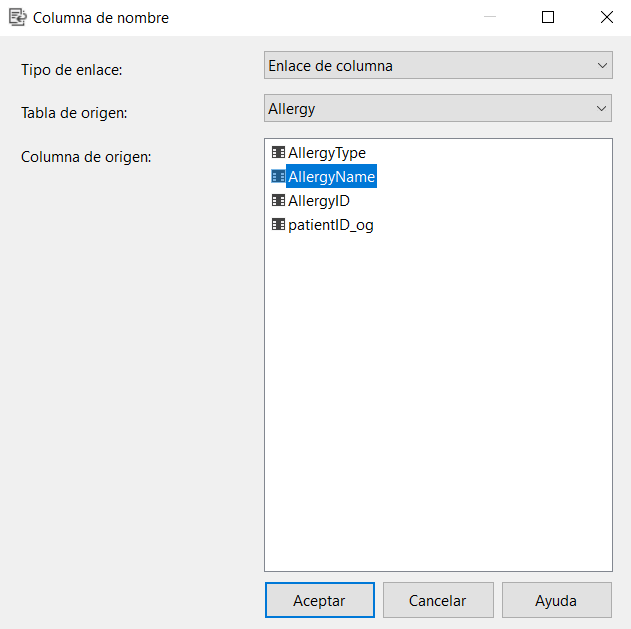
\includegraphics[width=1\textwidth]{image/allergyID}
	\caption{allergyID}
	\label{fig:19}
\end{figure}

Seleccionamos \texttt{AllergyName}.

\subsubsection{Diagnosis}

\textbf{Jerarquía:}

\begin{figure}[H]
	\centering
	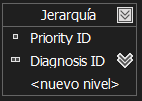
\includegraphics[width=0.5\textwidth]{image/JDiagnosis}
	\caption{Jerarquía de Diagnosis}
	\label{fig:20}
\end{figure}

\textbf{ValueColumn} y \textbf{NameColumn}:

\begin{figure}[H]
	\centering
	\includegraphics[width=1\textwidth]{image/DiagnosisID}
	\caption{DiagnosisID}
	\label{fig:21}
\end{figure}

Seleccionamos \texttt{DiagnosisString}.

\subsubsection{Medication}

\textbf{Jerarquía:}

\begin{figure}[H]
	\centering
	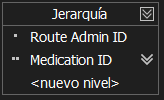
\includegraphics[width=0.5\textwidth]{image/JMedication}
	\caption{Jerarquía de Hospital}
	\label{fig:22}
\end{figure}

\textbf{ValueColumn} y \textbf{NameColumn} para \texttt{RouteAdminID}:

\begin{figure}[H]
	\centering
	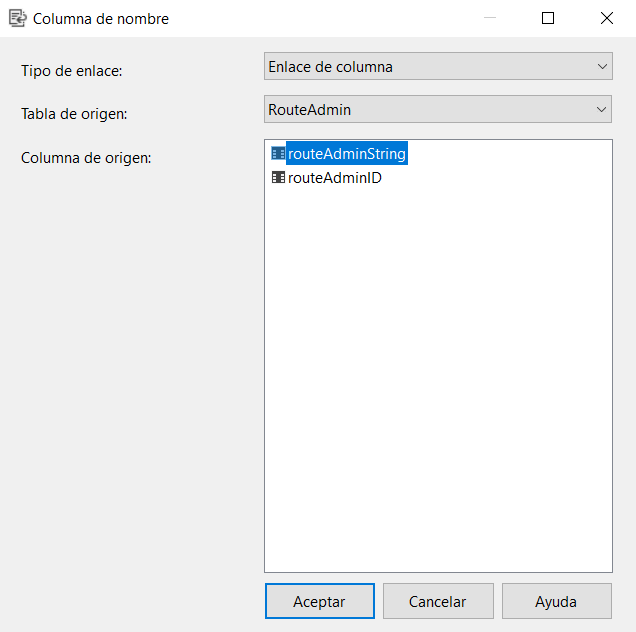
\includegraphics[width=1\textwidth]{image/routeAdmin}
	\caption{RouteAdminID}
	\label{fig:23}
\end{figure}

Seleccionamos \texttt{routeAdminString}.

\textbf{ValueColumn} y \textbf{NameColumn} para \texttt{MedicationID}:

\begin{figure}[H]
	\centering
	\includegraphics[width=1\textwidth]{image/MedicationID}
	\caption{MedicationID}
	\label{fig:24}
\end{figure}

Seleccionamos \texttt{DrugName}.

\subsubsection{Tiempo}

Para la dimensión Tiempo, será necesario primero arrastrar los atributos \texttt{HospitalDischargeTime24} y \texttt{HospitalDischargeYear} de la vista del origen de datos al apartado de atributos. Luego, arrastraremos primero \texttt{Year} y luego \texttt{Time24}, para tener dentro de los años las horas de ingreso asociadas.

Quedando algo parecido a la Figura \ref{fig:28}:

\begin{figure}[H]
	\centering
	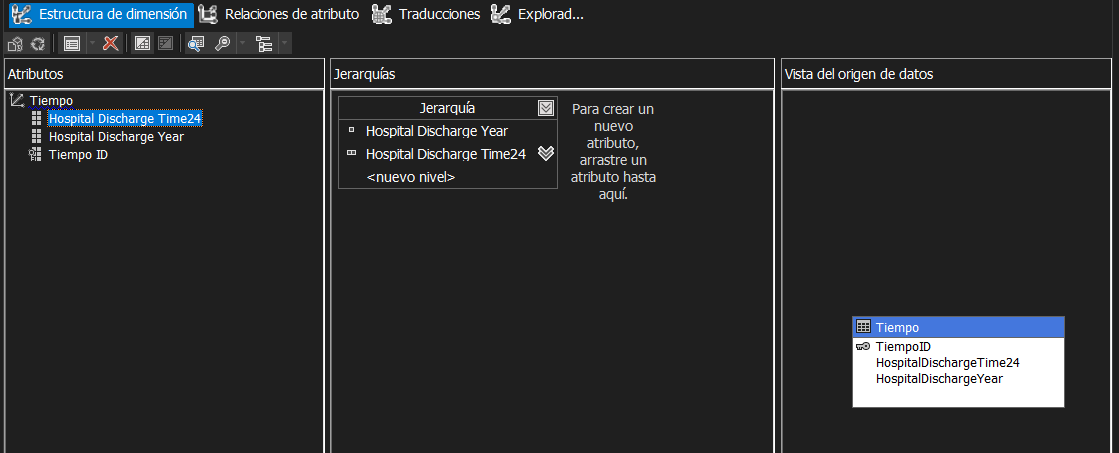
\includegraphics[width=1\textwidth]{image/JTiempo}
	\caption{Jerarquía de Tiempo}
	\label{fig:28}
\end{figure}

Posteriormente, para evitar errores de valor duplicado en la hora, haremos lo siguiente:

1. Daremos clic en el atributo \texttt{HospitalDischargeTime24}.

2. En el apartado de propiedades, seleccionaremos los tres puntos en \textbf{keyColumns}.

\begin{figure}[H]
	\centering
	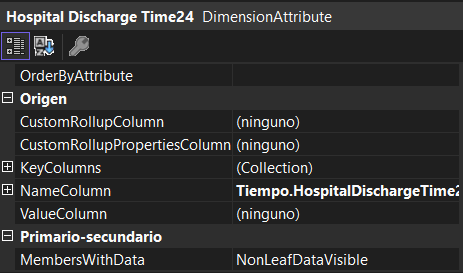
\includegraphics[width=1\textwidth]{image/tiempoPropiedades}
	\caption{Propiedades de Tiempo}
	\label{fig:25}
\end{figure}

Seleccionaremos las columnas \texttt{HospitalDischargeYear} y \texttt{HospitalDischargeTime24} para crear juntas una clave única. Con esto, aunque se repitan las horas, estarán vinculadas a un año, impidiendo el error de clave duplicada.

En \textbf{NameColumn}, seleccionaremos \texttt{HospitalDischargeTime24}. Esto es obligatorio, ya que en \textbf{keyColumn} tenemos dos claves y hay que especificar el nombre de la columna sobre la que trabajamos.

\begin{figure}[H]
	\centering
	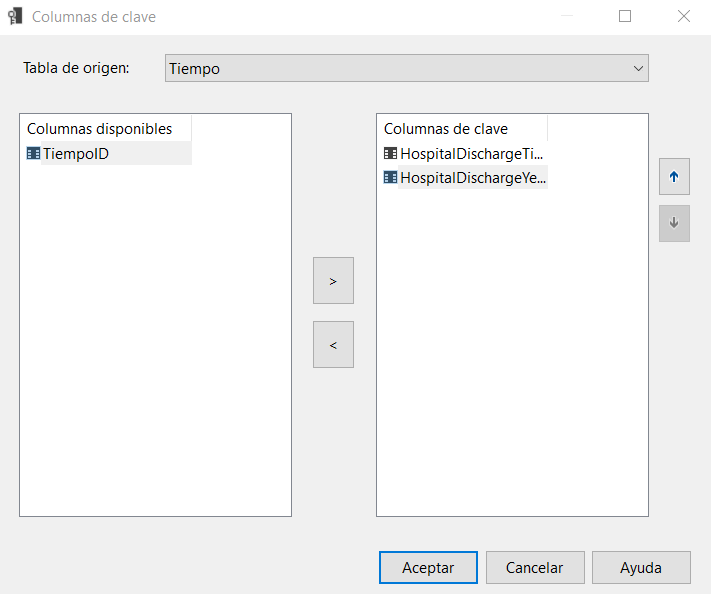
\includegraphics[width=1\textwidth]{image/keyColumnTiempo}
	\caption{Propiedades de Tiempo}
	\label{fig:29}
\end{figure}

Finalmente, en el apartado de \textbf{relaciones de atributo} dentro de la dimensión Tiempo, eliminaremos la relación entre \texttt{TiempoID} y \texttt{HospitalDischargeYear}, dando clic derecho y seleccionando "Eliminar".

\begin{figure}[H]
	\centering
	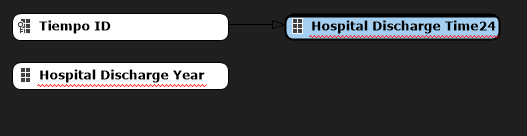
\includegraphics[width=1\textwidth]{image/relacionesTiempoDps1}
	\caption{Relaciones de Tiempo Antes}
	\label{fig:26}
\end{figure}

Luego, crearemos una nueva relación de atributo para \texttt{HospitalDischargeTime24}. Esto generará una configuración como la Figura \ref{fig:27}.

\begin{figure}[H]
	\centering
	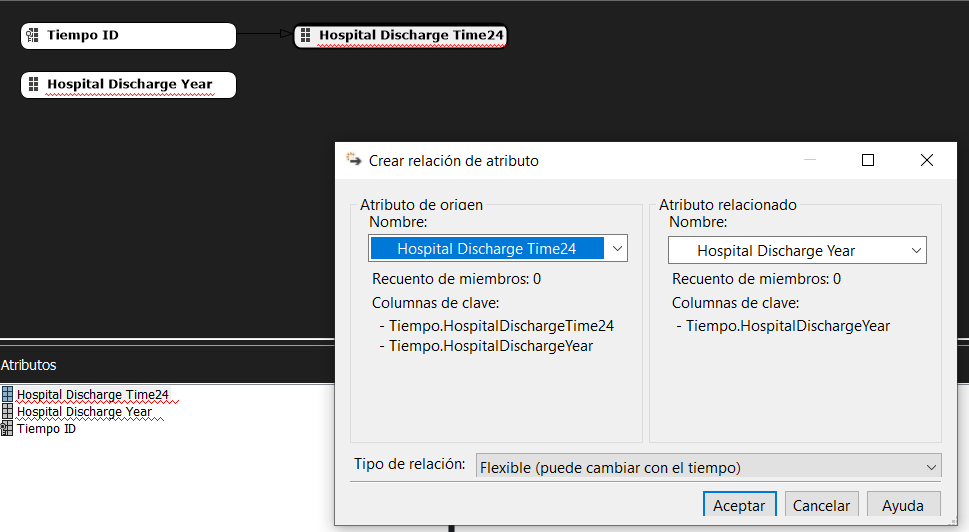
\includegraphics[width=1\textwidth]{image/relacionesTiempoDps2}
	\caption{Relaciones de Tiempo Después}
	\label{fig:27}
\end{figure}

Procedemos a darle a aceptar, y con ello habremos construido una jerarquía correctamente definida para \texttt{Tiempo}.


\subsection{Modificaciones del cubo}

Antes de desplegar el cubo 

	 \subsection{Instrucciones para desplegar el proyecto en el equipo}
	 
	 Para ejecutar la tarea, será suficiente con descomprimir el archivo. A continuación, se deberá hacer clic derecho sobre el proyecto multidimensional y seleccionar la opción ``Propiedades''. Una vez en el apartado de propiedades, se procederá a acceder a la sección de implementación, donde se deberá seleccionar el servidor correspondiente. En este caso, se podrá elegir como servidor `localhost` o bien `localhost\textbackslash nuestroServidorSQL`. En mi situación particular, dado que disponía de dos instancias de `MSSQLSERVER`, fue necesario especificar que se utilizaría la instancia `MSSQLSERVER2`, que es la que posee la funcionalidad multidimensional.
	 
	 \begin{figure}[H]
	 	\centering
	 	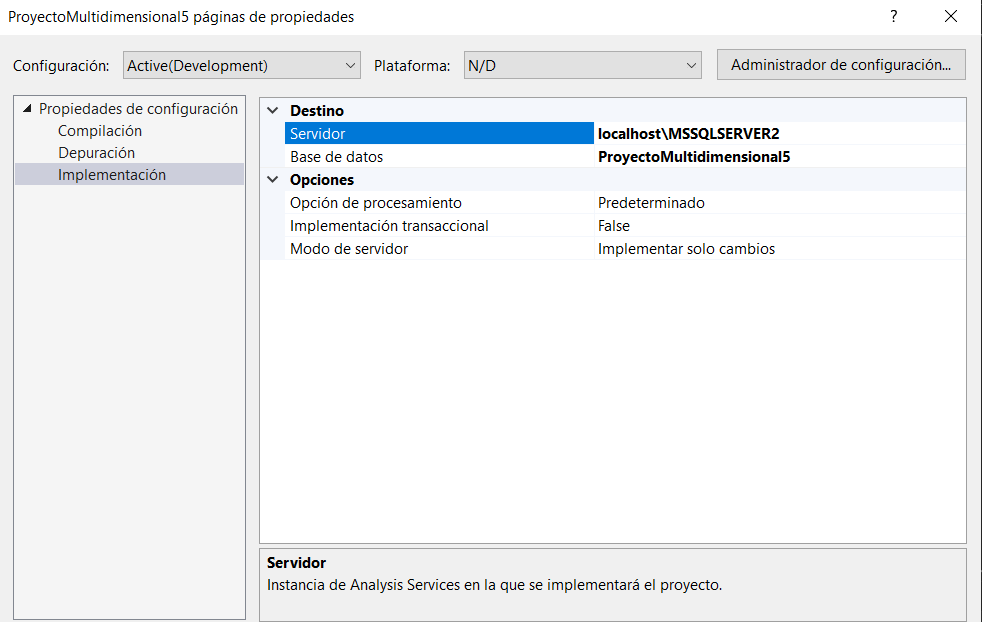
\includegraphics[width=1\textwidth]{image/despliegue}
	 	\caption{Configuración de despliegue}
	 	\label{fig:3}
	 \end{figure}
	 
	 Una vez configurado todo correctamente, se procederá a hacer clic en ``Iniciar'' y el proceso se completará de manera satisfactoria. 
	 
	Posteriormente, iniciaremos los servicios de Análisis (Analysis Services) en SQL Server Management Studio y verificaremos que tanto el proyecto \textit{ProyectoMultidimensional5} como el cubo se han desplegado correctamente.
	
	 
	
	\section{Consultas en MDX}
	- Una sección con las consultas en MDX y una captura con el resultado de cada una de ellas (la imagen capturada no tiene por qué mostrar todas las tuplas resultantes). 
	
	
	\section{Instrucciones para ejecutar las consultas.}
	- Una sección con las instrucciones detalladas para que un evaluador pueda ejecutar las consultas en su máquina. 
	
	
		- Para cada consulta MDX, se muestra, además del enunciado de la consulta en sí, la consulta realizada en MDX y una captura del resultado generado.
	
	- Indica el número de consultas MDX que se han intentando, es decir, que se ha escrito código MDX y se ha mostrado el resultado de la misma, independientemente de si son correctas o no:
	
	(***) 8 o más.
	
	
	- Según tu experiencia, valora cómo están realizadas las consultas en MDX, seleccionando la opción más adecuada:
	
	(****) Todas las consultas parecen ser correctas, teniendo sentido la salida de cada una de ellas. 
	
	
	- En algunas consultas se han usado funciones más avanzada de MDX, que impliquen el uso de métodos para recorrer una jerarquía (PREVMEMBER, CURRENTMEMBER, PARENT, etc.). 

	\section{Problemas encontrados}

	Entre los principales problemas que encontramos, destaca la conexión con la base de datos, la cual generaba errores de manera constante debido a que el método de autenticación no era configurado para utilizar \textit{SQL Authentication}.
	
	Adicionalmente, surgieron problemas derivados de un proceso de ETL incorrectamente implementado, lo que resultó en la presencia de múltiples tuplas con valores duplicados, como ocurrió en la tabla \textit{ingresoUCI} inicialmente.
	
	Aunque no se considera un problema en sentido estricto, decidimos modificar el atributo \textit{age}, cambiando su tipo de dato a \textit{int} para facilitar su utilización en las consultas, dado que este atributo es de gran utilidad.
	
	Finalmente, también se presentaron inconvenientes durante el proceso de despliegue, ya que se nos pasaba por alto que, con cada cambio realizado, era necesario procesar y actualizar el cubo.
	

	\section{Conclusión}
	
	XD


	\section{Github y conjunto de instrucciones para su correcto despliegue en SQL Server.}

	Todo el proyecto está accesible en github \cite{depab2024} donde se detalla más específicamente como desplegar en SQL.
	%%%%%%%%%%%%%%%%%%%%%%%%%%%%%%%%%%%%%%%%%%%%%%%%%%%%%%%%%%%%%%%%%%%%%%%%%%%
	\printbibliography
	
	
	%% Back Cover
	
\includepdf[noautoscale=true, width=\paperwidth]{backcover.pdf}
	
\end{document}